% Options for packages loaded elsewhere
\PassOptionsToPackage{unicode}{hyperref}
\PassOptionsToPackage{hyphens}{url}
\PassOptionsToPackage{dvipsnames,svgnames,x11names}{xcolor}
%
\documentclass[
  letterpaper,
  DIV=11,
  numbers=noendperiod]{scrartcl}

\usepackage{amsmath,amssymb}
\usepackage{iftex}
\ifPDFTeX
  \usepackage[T1]{fontenc}
  \usepackage[utf8]{inputenc}
  \usepackage{textcomp} % provide euro and other symbols
\else % if luatex or xetex
  \usepackage{unicode-math}
  \defaultfontfeatures{Scale=MatchLowercase}
  \defaultfontfeatures[\rmfamily]{Ligatures=TeX,Scale=1}
\fi
\usepackage{lmodern}
\ifPDFTeX\else  
    % xetex/luatex font selection
\fi
% Use upquote if available, for straight quotes in verbatim environments
\IfFileExists{upquote.sty}{\usepackage{upquote}}{}
\IfFileExists{microtype.sty}{% use microtype if available
  \usepackage[]{microtype}
  \UseMicrotypeSet[protrusion]{basicmath} % disable protrusion for tt fonts
}{}
\makeatletter
\@ifundefined{KOMAClassName}{% if non-KOMA class
  \IfFileExists{parskip.sty}{%
    \usepackage{parskip}
  }{% else
    \setlength{\parindent}{0pt}
    \setlength{\parskip}{6pt plus 2pt minus 1pt}}
}{% if KOMA class
  \KOMAoptions{parskip=half}}
\makeatother
\usepackage{xcolor}
\setlength{\emergencystretch}{3em} % prevent overfull lines
\setcounter{secnumdepth}{-\maxdimen} % remove section numbering
% Make \paragraph and \subparagraph free-standing
\ifx\paragraph\undefined\else
  \let\oldparagraph\paragraph
  \renewcommand{\paragraph}[1]{\oldparagraph{#1}\mbox{}}
\fi
\ifx\subparagraph\undefined\else
  \let\oldsubparagraph\subparagraph
  \renewcommand{\subparagraph}[1]{\oldsubparagraph{#1}\mbox{}}
\fi


\providecommand{\tightlist}{%
  \setlength{\itemsep}{0pt}\setlength{\parskip}{0pt}}\usepackage{longtable,booktabs,array}
\usepackage{calc} % for calculating minipage widths
% Correct order of tables after \paragraph or \subparagraph
\usepackage{etoolbox}
\makeatletter
\patchcmd\longtable{\par}{\if@noskipsec\mbox{}\fi\par}{}{}
\makeatother
% Allow footnotes in longtable head/foot
\IfFileExists{footnotehyper.sty}{\usepackage{footnotehyper}}{\usepackage{footnote}}
\makesavenoteenv{longtable}
\usepackage{graphicx}
\makeatletter
\def\maxwidth{\ifdim\Gin@nat@width>\linewidth\linewidth\else\Gin@nat@width\fi}
\def\maxheight{\ifdim\Gin@nat@height>\textheight\textheight\else\Gin@nat@height\fi}
\makeatother
% Scale images if necessary, so that they will not overflow the page
% margins by default, and it is still possible to overwrite the defaults
% using explicit options in \includegraphics[width, height, ...]{}
\setkeys{Gin}{width=\maxwidth,height=\maxheight,keepaspectratio}
% Set default figure placement to htbp
\makeatletter
\def\fps@figure{htbp}
\makeatother

\KOMAoption{captions}{tableheading}
\makeatletter
\@ifpackageloaded{caption}{}{\usepackage{caption}}
\AtBeginDocument{%
\ifdefined\contentsname
  \renewcommand*\contentsname{Table of contents}
\else
  \newcommand\contentsname{Table of contents}
\fi
\ifdefined\listfigurename
  \renewcommand*\listfigurename{List of Figures}
\else
  \newcommand\listfigurename{List of Figures}
\fi
\ifdefined\listtablename
  \renewcommand*\listtablename{List of Tables}
\else
  \newcommand\listtablename{List of Tables}
\fi
\ifdefined\figurename
  \renewcommand*\figurename{Figure}
\else
  \newcommand\figurename{Figure}
\fi
\ifdefined\tablename
  \renewcommand*\tablename{Table}
\else
  \newcommand\tablename{Table}
\fi
}
\@ifpackageloaded{float}{}{\usepackage{float}}
\floatstyle{ruled}
\@ifundefined{c@chapter}{\newfloat{codelisting}{h}{lop}}{\newfloat{codelisting}{h}{lop}[chapter]}
\floatname{codelisting}{Listing}
\newcommand*\listoflistings{\listof{codelisting}{List of Listings}}
\makeatother
\makeatletter
\makeatother
\makeatletter
\@ifpackageloaded{caption}{}{\usepackage{caption}}
\@ifpackageloaded{subcaption}{}{\usepackage{subcaption}}
\makeatother
\ifLuaTeX
  \usepackage{selnolig}  % disable illegal ligatures
\fi
\usepackage{bookmark}

\IfFileExists{xurl.sty}{\usepackage{xurl}}{} % add URL line breaks if available
\urlstyle{same} % disable monospaced font for URLs
\hypersetup{
  pdftitle={Comparing the Pittsburgh Steelers under Bill Cowher vs.~Mike Tomlin},
  colorlinks=true,
  linkcolor={blue},
  filecolor={Maroon},
  citecolor={Blue},
  urlcolor={Blue},
  pdfcreator={LaTeX via pandoc}}

\title{Comparing the Pittsburgh Steelers under Bill Cowher vs.~Mike
Tomlin}
\author{}
\date{}

\begin{document}
\maketitle

\begin{center}

STAT184 Final Project

JJ Steinbugl and Sammit Bal

12/18/2024

\end{center}

\textbf{Introduction}

The Pittsburgh Steelers are one of the most famous franchises in NFL
history, known for their iconic players, championship success, and
leadership. Over the past three decades, the team has been shaped by two
head coaches: Bill Cowher and Mike Tomlin.

Bill Cowher, who coached the team from 1992 to 2006, is known for his
strong defensive-minded strategies, and running focused offence. Under
his leadership, the Steelers reached the Super Bowl twice, winning in
2005. Following Cowher's tenure, Mike Tomlin took the reins in 2007,
becoming the youngest head coach to win a Super Bowl in 2008.

In this report we will compare the Steelers' performance under Cowher
and Tomlin, exploring their impact on the franchise through various
metrics, including win-loss records, playoff consistency, and average
offensive and defensive rankings. Additionally, we will consider how
changes in the NFL's playstyle may have influenced their respective
coaching tenures.

This analysis aims to answer a few critical questions about who has been
the better coach, who demonstrated greater consistency, and who achieved
more success during their time at the helm of the Pittsburgh Steelers?

\textbf{Methodology}

This analysis compares the performance of the Pittsburgh Steelers under
Bill Cowher (1992--2006) and Mike Tomlin (2007--present). The following
outlines the approach taken to gather, analyze, and interpret data, as
well as the methods used to account for changes in NFL playstyles over
time.

Data was gathered from Pro Football Reference, and Statista, this data
includes win-loss records, divisional rankings, offensive and defensive
rankings, and points scored and allowed. After the data was gathered we
cleaned and merged the data sources in order to consolidate our data and
make it easier to work with in the future. The data also meets the FAIR
principles as it can be easily found, it is accessible and free to
download, it can be easily interpreted in CSV format, and it can easily
be reused.

We recognize that football is an ever evolving sport and understand how
NFL rule changes can affect a teams playstyle. Over the years we have
noticed the shift toward pass-heavy offenses and rule changes favoring
offensive play and player safety. To address these changes, the analysis
will consider and address these recent trends/changes before any type of
conclusion is made.

\textbf{Research Questions:}

\begin{itemize}
\item
  Who is the better coach for the Pittsburgh Steelers?
\item
  Who is more consistent in their rankings during their tenure?
\item
  Who was more successful during their tenure?
\item
  How does the evolving NFL playstyle affect the statistics?
\end{itemize}

\textbf{Analysis:}

Graphical Comparisons: Include and interpret the graphs you created.
Break these down by tenure, rankings, success metrics, and consistency.
Evolving NFL Playstyle: Discuss trends in the league (e.g., changes in
offensive/defensive styles) and their possible impact on the coaches'
statistics. Discussion:

Address each research question in detail, supported by the data and
insights from the graphs. Discuss any limitations in your analysis,

\begin{itemize}
\item
  Who is the better coach for the Pittsburgh Steelers?

  This is the obvious question to ask in this analysis, but is indeed
  the overarching question. We will first analyze wins and losses, as it
  is the first thing you think of when you think of a coach.

  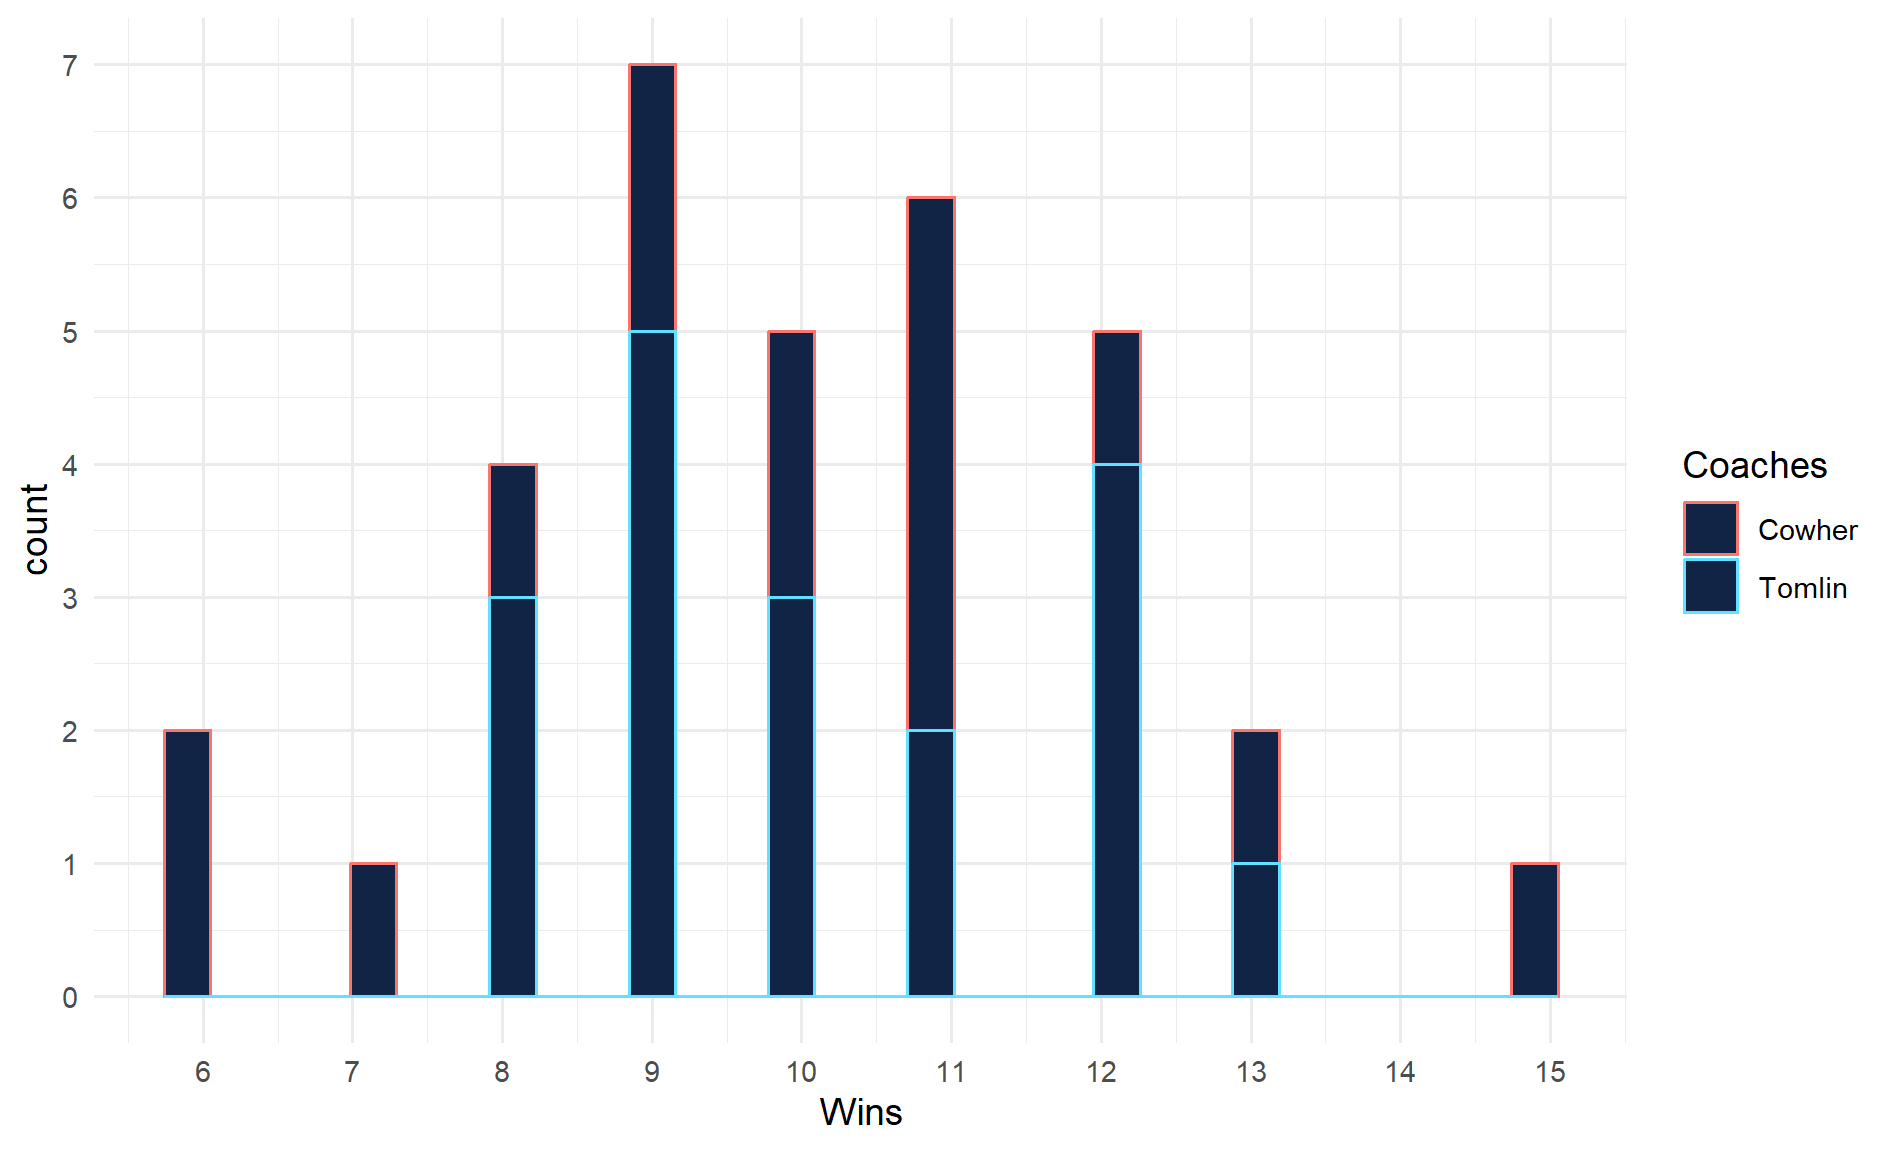
\includegraphics{images/clipboard-4000230535.png}

  This is a graph that shows through their time as a coach how many
  times Coaches Cowher and Tomlin got a certain amount of wins. These
  counts range from 6 to 15, with Cowher taking the lowest and highest.
  We see that Mike Tomlin has been very consistent from the 8 to 13 win
  range, but Bill Cowher has had more variety in his win columns. An
  important note to consider here is that When Cowher coached, there
  were only 16 games in the season, as opposed to Tomlin who has 17
  games in each season. We interpret that Tomlin has been much more
  consistent with winning, but we are aware of the uneven game amounts.

  The next category we analyzed was each coaches total points scored in
  terms of both their wins and their points scored. The graph comparing
  points scored to wins is on the left, and the one comparing points
  scored to the year is on the right.

  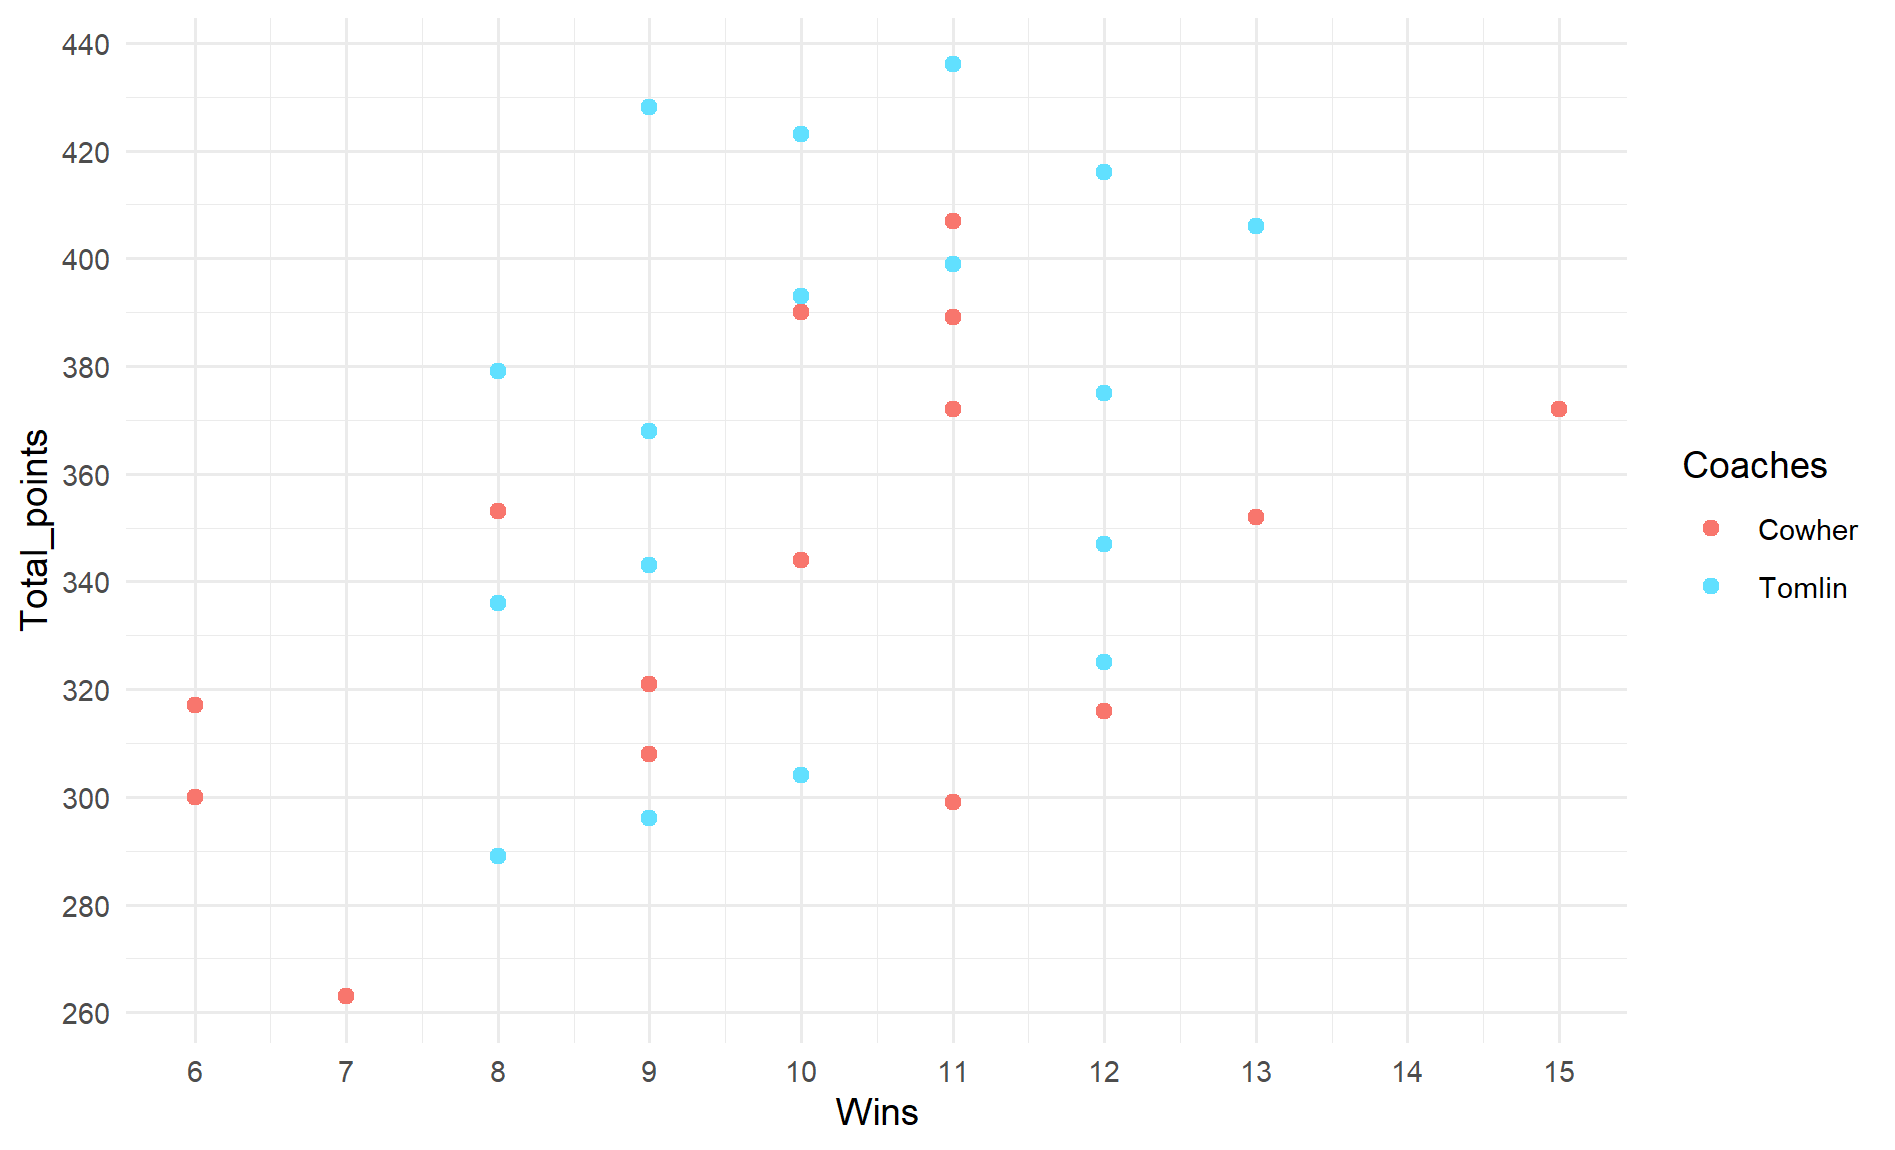
\includegraphics{images/clipboard-3424389474.png}

  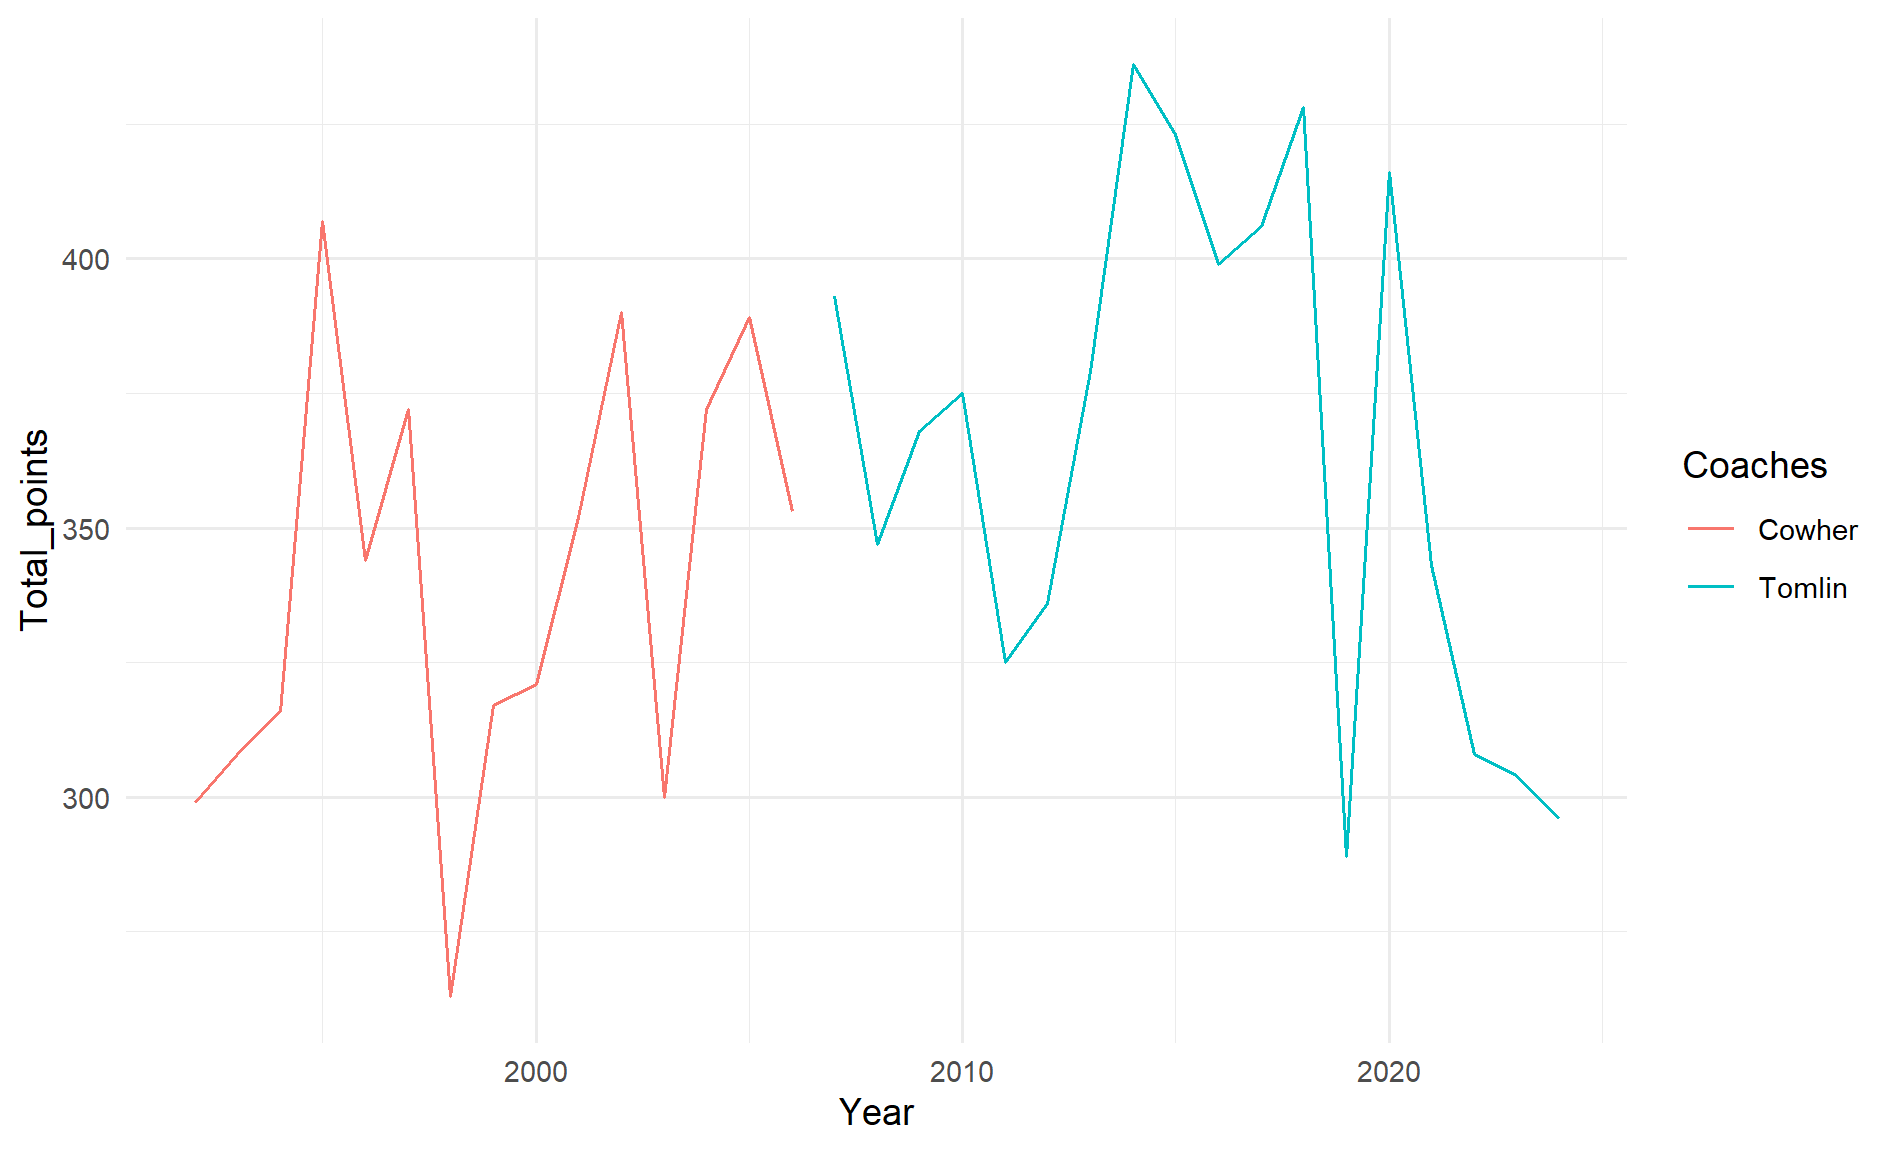
\includegraphics{images/clipboard-64297739.png}

  As you can see, the graph on the right once again favors Tomlin, as he
  is much more consistently scoring points, which by correlation is
  going to contribute to winning more games, as we saw in the graph
  above. But, a trend that has appeared in the more recent years of the
  NFL is that NFL football is a much higher scoring game than in years
  past. This is easily seen in the graph on the right, as Tomlin is
  easily scoring more points than Cowher, even in his seasons with less
  wins.
\item
  Who is more consistent in their rankings during their tenure?

  The next thing we can look at is how these two coaches compared to
  their colleagues throughout their time coaching. We will analyze
  graphs comparing their ranks in all categories, offensive and
  defensive.

  The first visualization we made was comparing the offensive points
  scored ranking of the coaches each year they coached. In terms of
  ranking, number 1 is the best, so the lower the line is, the better
  the coach was ranked in that year.

  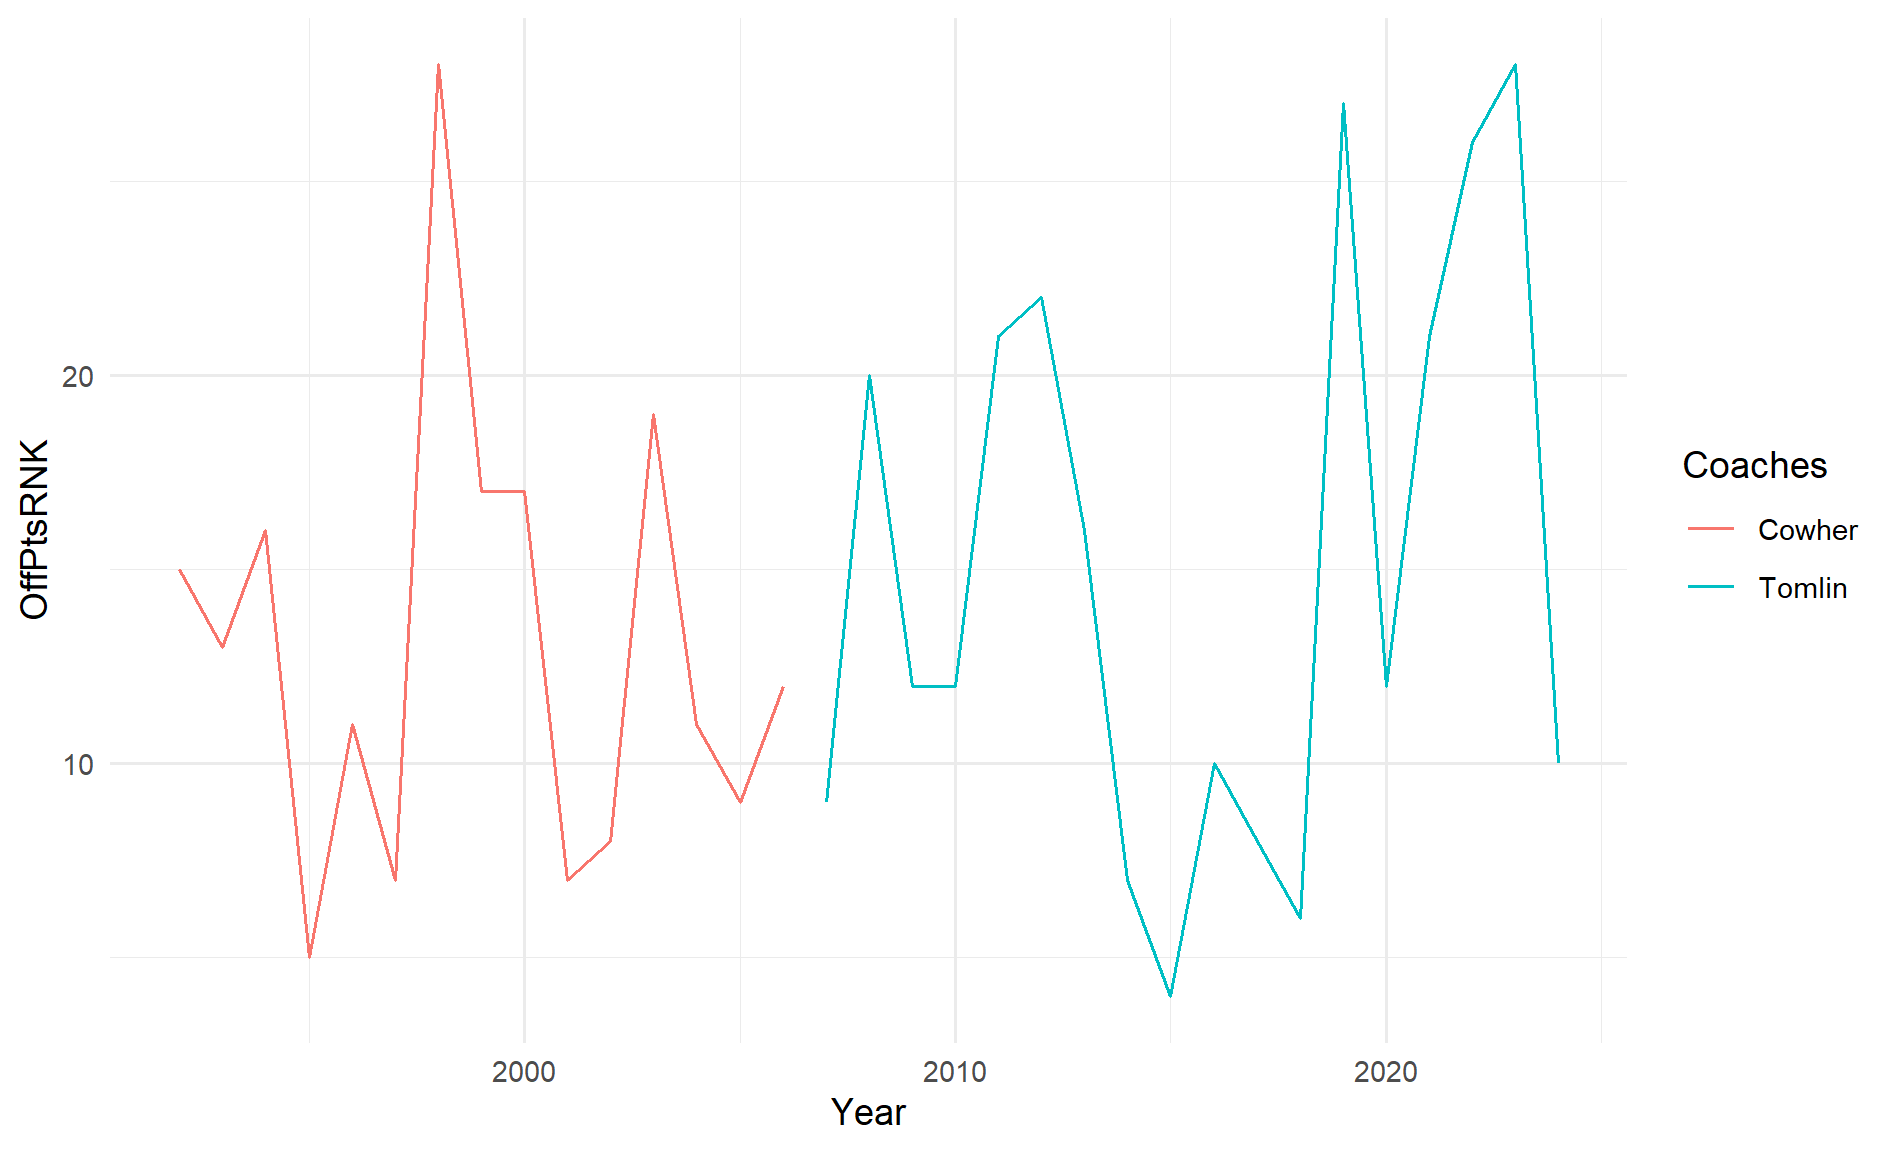
\includegraphics{images/clipboard-2906734705.png}

  In the graph we can see that Mike Tomlin is much more variable, having
  multiple spikes in rank up in the 20's, but a few short years close to
  2 or 3. Coach Cowher is more consistent, only having one big spike up
  in the high 20's, but other than that having a consistent rank of
  around 8.

  We then did the same for defensive points scored rank. The same rule
  that lower is better applies to this graph as well.

  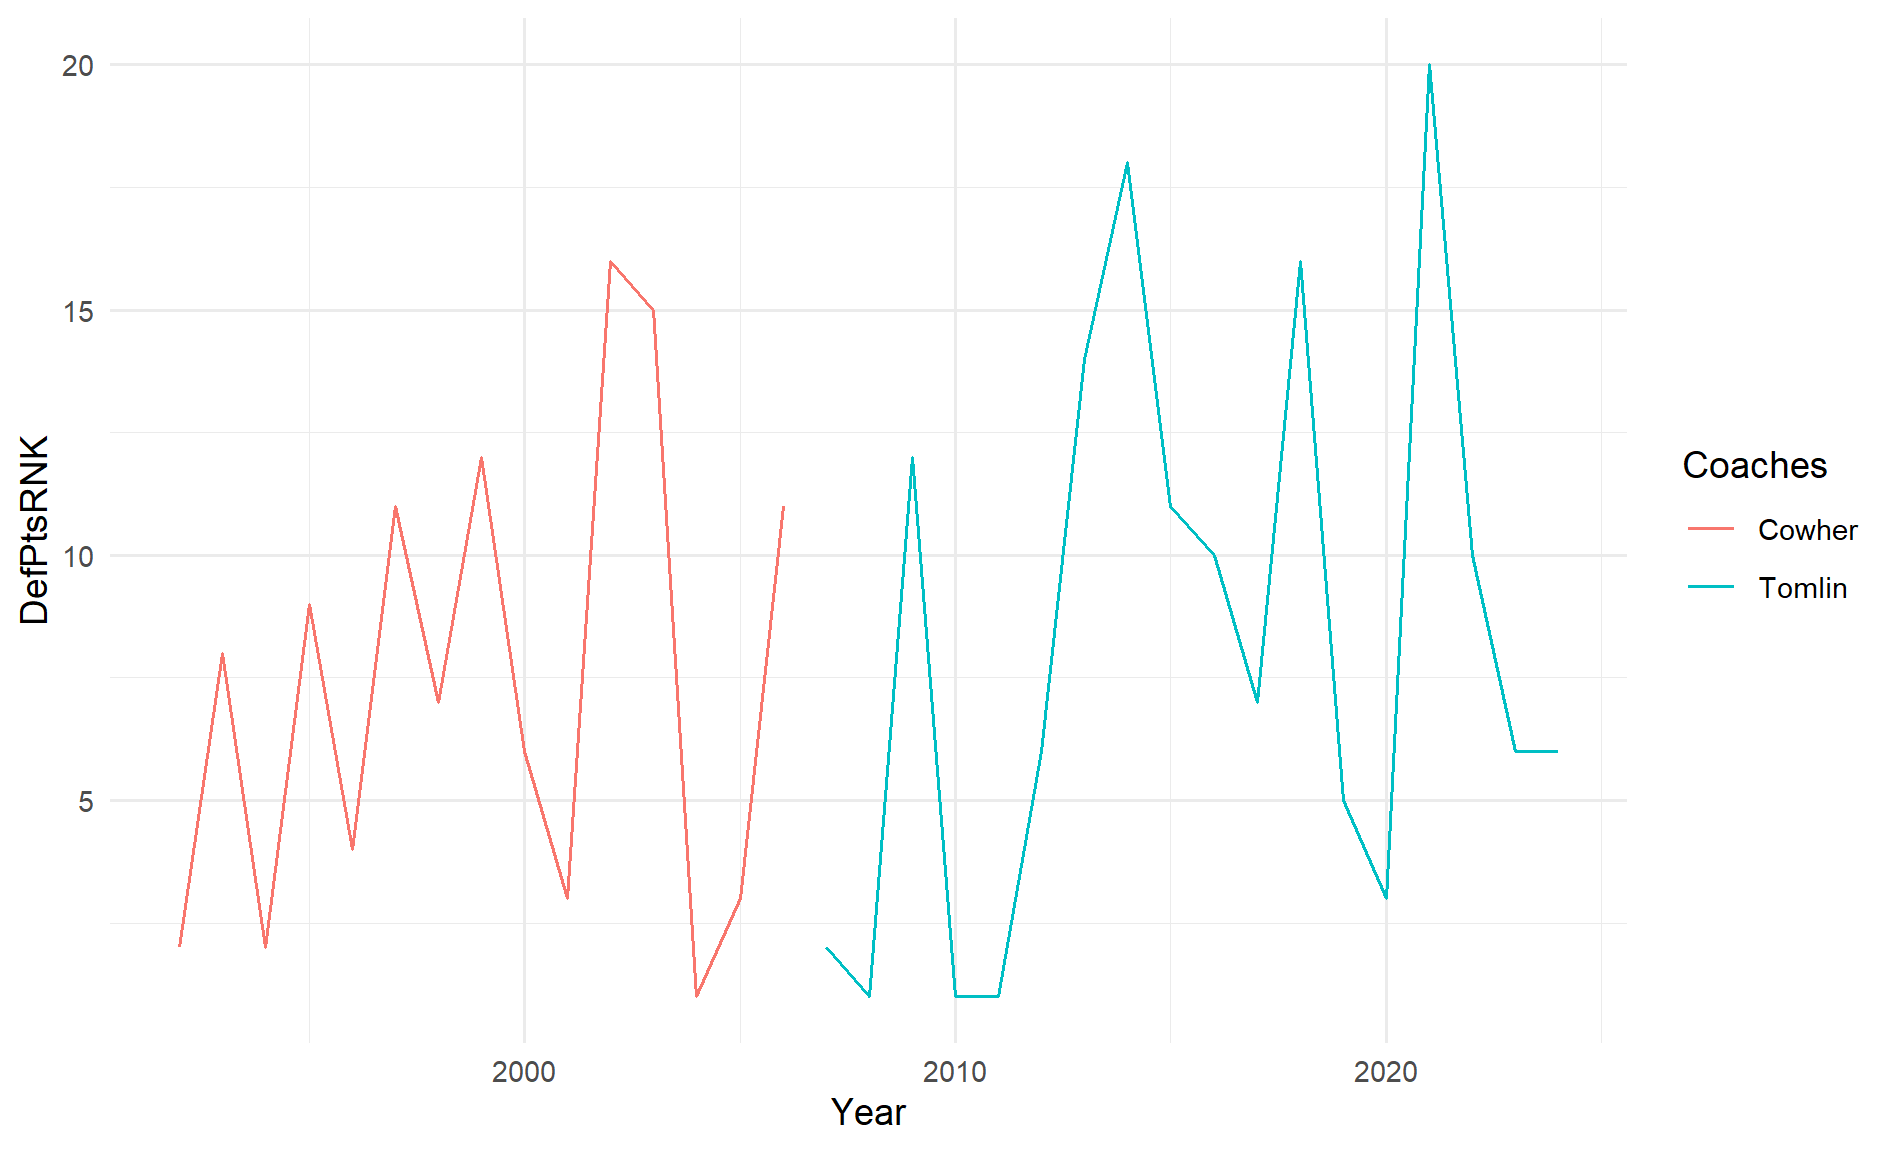
\includegraphics{images/clipboard-3632505765.png}

  From this graph we can see that Mike Tomlin is very sporadic with his
  rankings, some very high, and some very low, whereas Bill Cowher is
  much more consistent, with far less spikes than Tomlin.

  The next graph shows the coaches rank in terms of offensive and
  defensive yards. In this particular graph, the further in the bottom
  left the coach is, the better their ranks were.

  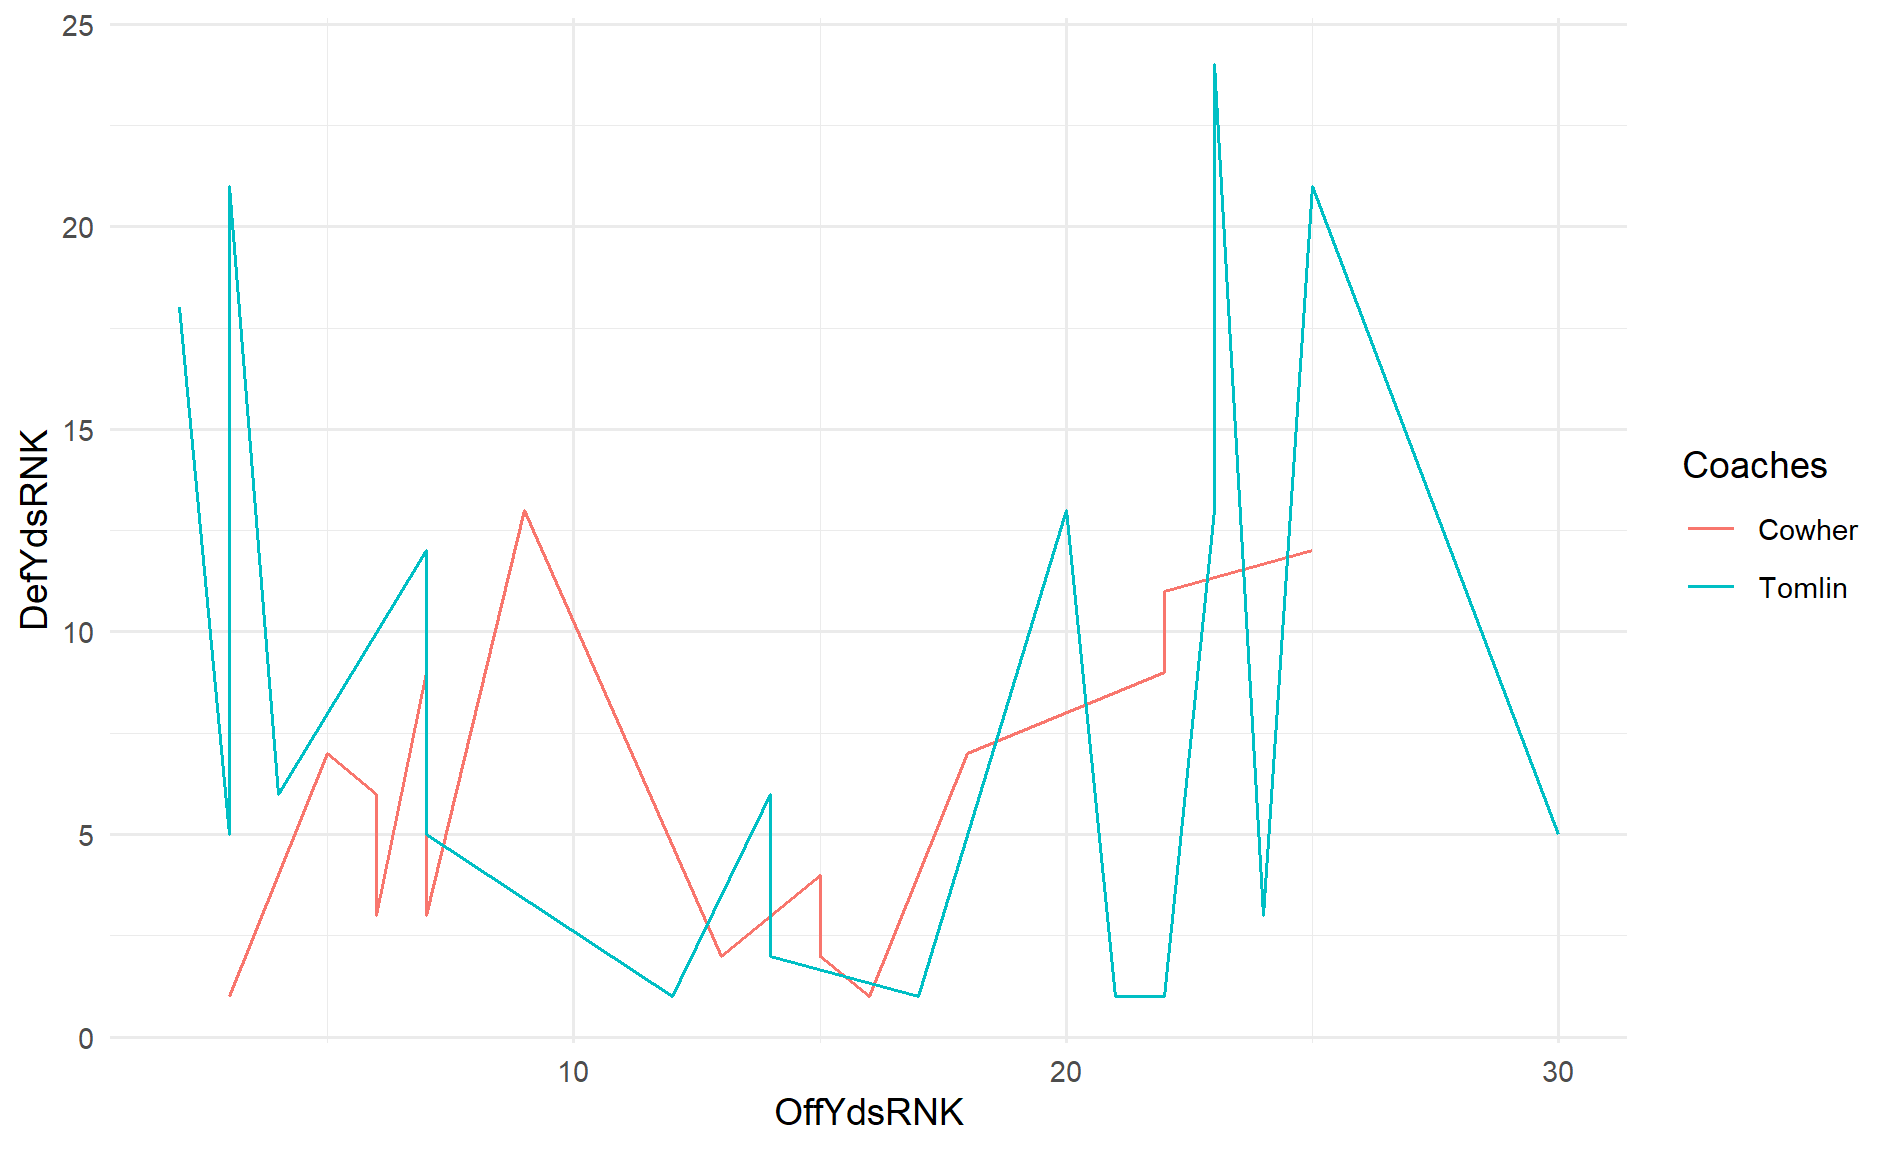
\includegraphics{images/clipboard-3198986412.png}

  We can see that Coach Cowher was able to acquire much lower ranks in
  both offensive and defensive yards. We can also see that he was much
  more consistent in his time, keeping all of his ranks low whereas Mike
  Tomlin had years with very high ranks.
\item
  Who was more successful during their tenure?

  When determining success, one of the most common standpoints to view
  success is by end of the season ranks, as well as playoff runs. We
  will compare both of these to see the success level of each coach.

  Our first graph is comparing the divisional finishes. One thing we
  have to be aware of is that in Cowher's time, there were 5 and 6 teams
  in the playoff, compared to the modern day 4 teams.

  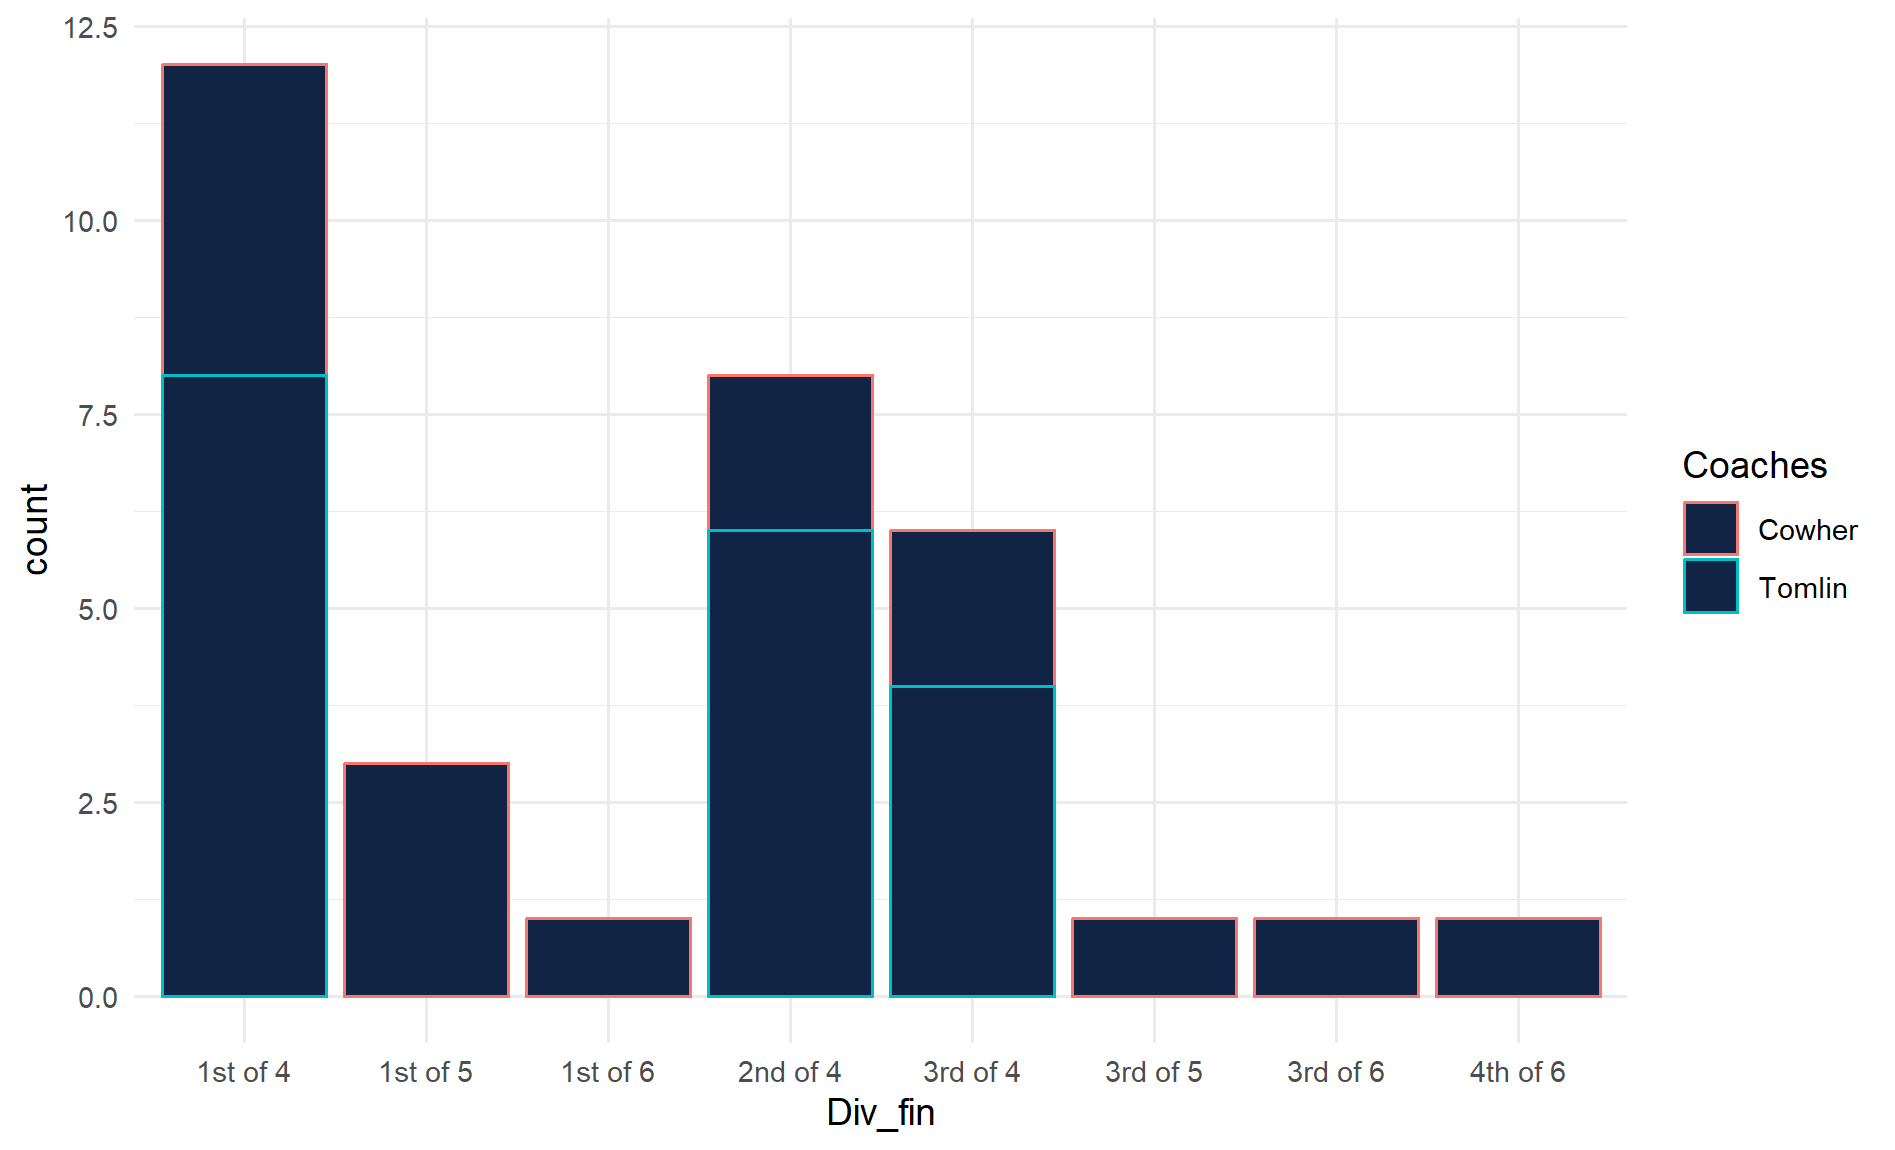
\includegraphics{images/clipboard-1894425753.png}

  Here we can see that accounting for the different amount of teams
  between the two time frames, the coaches are pretty even. Each coach
  has finished first about 7 times, and they have each finished second
  and third the same amount of times. This tells us they were both very
  successful, but nothing too prominent to distinguish them from one
  another.

  Now we can compare their playoff appearances, and to what level they
  got to. The order in terms of least important to most important is as
  follows:
\item
  No Appearance
\item
  Lost WC
\item
  Lost Div
\item
  Lost Conf
\item
  Lost SB
\item
  Won SB
\item
  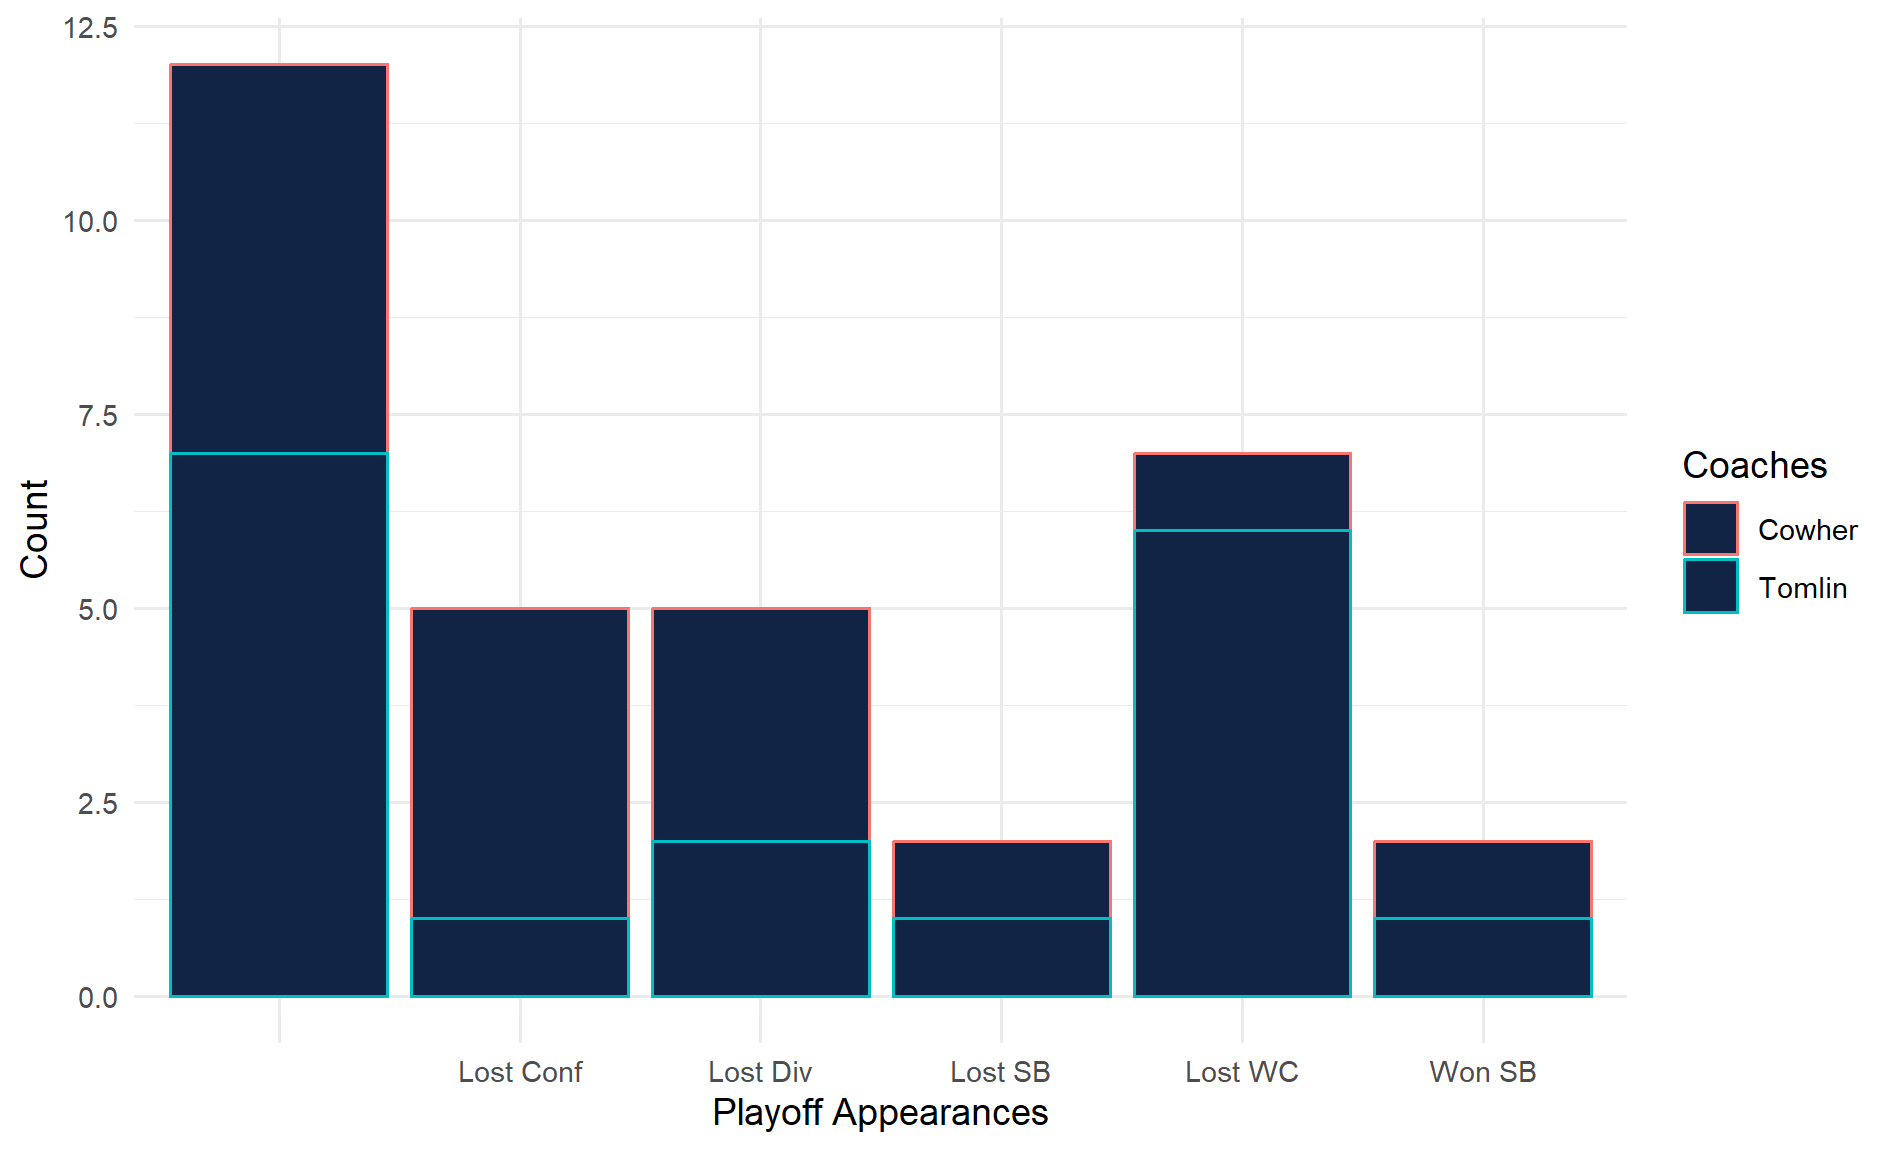
\includegraphics{images/clipboard-172469514.png}

  We observe that in terms of the most important appearance, the
  Superbowl, both coaches have won one and lost one, so there is no
  significant difference there. But, we do see that coach Cowher is
  leading in both the Lost Conf and Lost Div columns, meaning that he
  was able to get further in the playoffs a lot more often than coach
  Tomlin. From this we determine that Bill Cowher was more successful in
  the playoffs.
\item
  How does the evolving NFL playstyle affect the statistics?

  Earlier we discussed how the NFL gameplay has changed in terms of
  being higher scoring, as well as the changing of the divisions and how
  that might have some effect on how a coach's success is viewed. But
  the most underlying bias we found was in a metric some people might
  forget about when talking about football: money. Many people determine
  success on how much revenue a coach can bring in during their time.
\end{itemize}

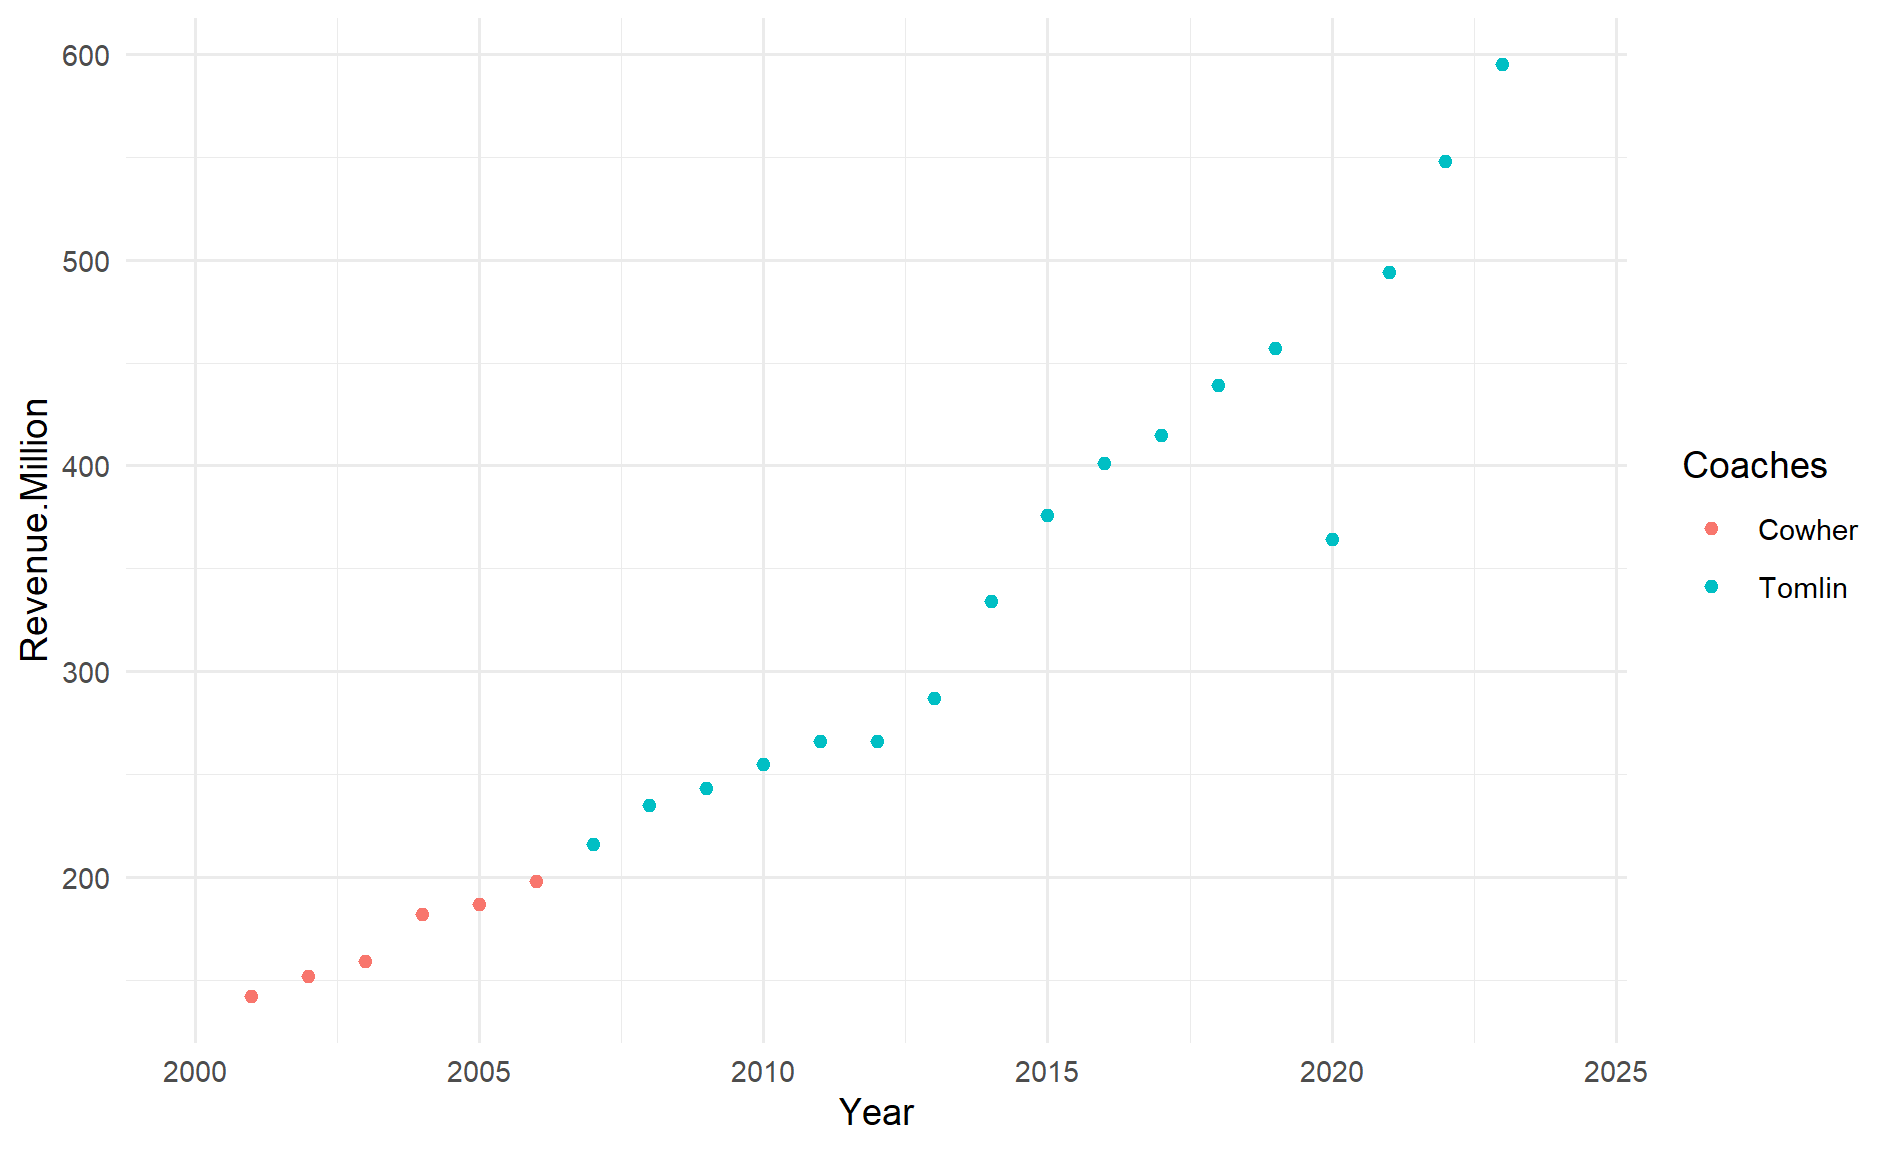
\includegraphics{images/clipboard-244220973.png}

At first glance, when looking at this graph, one might think that Tomlin
has blown Cowher out of the water in terms of revenue. In reality, if we
account for the underlying change in the way the NFL makes money as well
as the inflation rate in recent years, we actually find that Cowher made
more revenue per year than Tomlin when accounting for inflation.

\textbf{Conclusion}

When taking all of these graphs and conclusions into account, we
discover a couple things: In terms of winning and points scored, we see
that Mike Tomlin edges out Bill Cowher, even when accounting for a
higher scoring NFL and a different game than past years. But, in terms
of consistency, espeically in rankings, Bill Cowher is miles ahead in
almost every metric. In terms of success, both coaches have done very
well in their tenures, but Bill Cowher was able to finish just a little
higher than Mike Tomlin in both division finishes and playoff runs.

We understand that deciding who is the better coach is an objective
question, and at the end of the day an opinion, so the interpretations
of our graphs are layed out for the reader to make their own judgement.
Nevertheless, through our analysis, we conclude that Bill Cowher was
overall a better coach for the Pittsburgh Steelers.

\textbf{References}

Include all references used in report and analysis.

\section{\textless\textless\textless\textless\textless\textless\textless{}
HEAD}\label{head}

\textbf{Research Questions:}

\begin{itemize}
\item
  Who is the better coach for the Pittsburgh Steelers?
\item
  Who is more consistent in their rankings during their tenure?
\item
  Who was more successful during their tenure?
\item
  How does the evolving NFL playstyle affect the statistics?
\end{itemize}

test

\begin{quote}
\begin{quote}
\begin{quote}
\begin{quote}
\begin{quote}
\begin{quote}
\begin{quote}
8f32833812f3452b77e793e12c530608568d5306 \#\# Running Code
\end{quote}
\end{quote}
\end{quote}
\end{quote}
\end{quote}
\end{quote}
\end{quote}



\end{document}
